%\documentclass[12pt, handout]{beamer}
\documentclass[12pt]{beamer}

\usepackage{cmap}
\usetheme{Madrid}
\usepackage[utf8]{inputenc}
\usepackage[russian]{babel}
\usepackage[OT1]{fontenc}
\usepackage{amsmath}
\usepackage{amsfonts}
\usepackage{amssymb}
\usepackage{graphicx}
\usepackage{listings}

\author{Игорь Рязанцев}
\title{Функции и объекты в Python}
\institute{Лекция 02}
\date{2021г.}

%\setbeamercovered{transparent} 
\setbeamertemplate{navigation symbols}{} 
%\logo{} 
%\institute{} 
%\date{} 
%\subject{} 

\begin{document}

\begin{frame}
\titlepage
\end{frame}

\begin{frame}{Тестовое задание [Лекция 01]}
\textbf{\# Необходимо вывести наименование светильника c наибольшим световым потоком и наименьшей потребляемой мощностью} 
\vspace{0.5cm}
\lstinputlisting[language=Python]{code/17.py}
\vspace{0.5cm}
\end{frame}

\begin{frame}{Тестовое задание [Лекция 01]}
\lstinputlisting[language=Python]{code/18.py}
\vspace{0.5cm}
\end{frame}

\begin{frame}[t]{Оглавление}
\tableofcontents[part=1]
\end{frame}

%\begin{frame}[t]{Оглавление}
%\tableofcontents
%\end{frame}


\part{1}
\section{Функции}
\begin{frame}{Функции}
\textbf{Преимущества использования функций:}
\begin{itemize}
\item исключение дублирования кода;
\item многократное выполнение ранее написанного кода;
\item улучшение читаемости кода.
\end{itemize}
\end{frame}

\begin{frame}{Определение функции}
\textbf{\# Пример без функций:} \\
\vspace{0.5cm}
\lstinputlisting[language=Python]{code/19.py}
\vspace{0.5cm}
Результат: \\
Hello Word! \\
Hello Word! \\
\end{frame}


\subsection{Определение функции}
\begin{frame}{Определение функции}
\textbf{Функция -- именованный блок кода, предназначенный для решения одной конкретной задачи.} \\
\vspace{0.3cm}
\textbf{\# Пример c использованием функций:} \\
\vspace{0.2cm}
\lstinputlisting[language=Python]{code/20.py}
\vspace{0.5cm}
Результат: \\
Hello Word! \\
Hello Word! \\
\end{frame}


\subsection{Передача информации в функцию}
\begin{frame}{Передача информации в функцию}
\vspace{0.5cm}
\lstinputlisting[language=Python]{code/21.py}
\vspace{0.5cm}
Переменная username в определении greet\_user() -- \textit{параметр}, то есть условные данные, необходимые функции для выполнения ее работы. Значение Helen в greet\_user(\'Helen\') -- \textit{аргумент}, то есть конкретная информация, переданная при вызове функции.
\end{frame}


\begin{frame}{Передача информации в функцию}
Важен порядок передачи аргументов в функцию. \\Он должен совпадать с соответствующими принимающими параметрами. \\
\vspace{0.5cm}
\lstinputlisting[language=Python]{code/22.py}
\vspace{0.5cm}
Результат: \\
21 is Helen! \\
\end{frame}

\subsection{Именованные аргументы}
\begin{frame}{Именованные аргументы}
\textit{Именованный аргумент} представляет собой пару <<имя-значение>>, передаваемую функции. Имя и значение связываются с аргументом напрямую. \\
\vspace{0.5cm}
\lstinputlisting[language=Python]{code/23.py}
\vspace{0.5cm}
Результат: \\
Helen is 21! \\
\end{frame}


\subsection{Значения по умолчанию}
\begin{frame}{Значения по умолчанию}
Если при вызове функции передается аргумент, соответствующий данному параметру, Python использует значение аргумента, а если нет — использует значение по умолчанию.\\
\vspace{0.5cm}
\lstinputlisting[language=Python]{code/24.py}
\vspace{0.5cm}
Результат: \\
Helen is 21! \\
\end{frame}


\subsection{Возвращаемое значение}
\begin{frame}{Возвращаемое значение}
\textbf{return} -- оператор возврата из функции с возможностью передачи значения.\\
\vspace{0.5cm}
\lstinputlisting[language=Python]{code/25.py}
\vspace{0.5cm}
Результат: \\
200 \\
\end{frame}


\begin{frame}{Возвращаемое значение}
Функция может вернуть любое значение, в том числе и более сложную структуру данных (например, список).\\
\vspace{0.2cm}
\lstinputlisting[language=Python]{code/26.py}
\end{frame}


\begin{frame}{Тестовое задание}
\textbf{\# Необходимо написать функцию вычисления факториала} \\
\vspace{0.5cm}
\textbf{Факториалом числа N} называется произведение всех чисел от единицы до N. \\
\vspace{0.1cm}
Например, 5! = 1*2*3*4*5 \\
\vspace{0.1cm}
Факториал нуля равен единице, как и факториал самой единицы: \\
0! = 1  1! = 1
\\Это нужно запомнить, и учесть в своей программе!
\vspace{0.5cm}
\end{frame}

\begin{frame}{Тестовое задание}
\vspace{0.2cm}
\lstinputlisting[language=Python]{code/27.py}
\vspace{0.5cm}
Результат: \\
120 \\
\end{frame}

\section{Импорт модулей}
\begin{frame}{Импорт модулей}
\textbf{Вариант 1}
\vspace{0.5cm}
\lstinputlisting[language=Python]{code/28.py}
\vspace{0.5cm}
Результат: \\
120 \\
\end{frame}


\begin{frame}{Импорт модулей}
\textbf{Вариант 2}
\vspace{0.5cm}
\lstinputlisting[language=Python]{code/29.py}
\vspace{0.5cm}
Результат: \\
120 \\
\end{frame}


\begin{frame}{Импорт модулей}
\textbf{Вариант 3}
\vspace{0.5cm}
\lstinputlisting[language=Python]{code/30.py}
\vspace{0.5cm}
Результат: \\
120 \\
\end{frame}

\section{Объектно-ориентированное программирование}
\begin{frame}[t]{Оглавление}
\tableofcontents[currentsection]
\end{frame}

\subsection{Создание класса}
\begin{frame}{Создание класса}
Класс определяет общее поведение для целой категории объектов. \textbf{Класс -- это спецификация}.
\lstinputlisting[language=Python]{code/31.py}
\end{frame}

\subsection{Создание экземпляра класса}
\begin{frame}{Создание экземпляра класса}
Создание объекта на основе класса называется \textbf{созданием экземпляра класса}
\vspace{0.5cm}
\lstinputlisting[language=Python]{code/31_1.py}
\vspace{0.5cm}
Результат: \\
LED is switch on!\\
\end{frame}

\subsection{Обращение к методам}
\begin{frame}{Обращение к методам}
\begin{itemize}
\item Функция, являющаяся частью класса, называется \emph{методом}.
\item Параметр \emph{self} обязателен в определении метода; он должен предшествовать всем остальным параметрам.
\item Поведение методов аналогично функциям. Отличие состоит в вызове метода (<<точечная>> запись):
\\
\vspace{0.5cm}
\textbf{экземпляр\_класса.метод()} \\
\vspace{0.5cm}
\lstinputlisting[language=Python]{code/31_2.py}
\vspace{0.5cm}
\end{itemize}
\end{frame}


\subsection{Обращение к атрибутам}
\begin{frame}{Обращение к атрибутам}
Для обращения к атрибутам экземпляра используется <<точечная>> запись.
\vspace{0.5cm}
\lstinputlisting[language=Python]{code/31_3.py}
\vspace{0.5cm}
Результат: \\
LED is switch on!\\
LED is switch on!\\
\end{frame}


\begin{frame}{Назначение атрибуту значения по умолчанию}
Каждый атрибут класса должен иметь исходное значение, даже если оно равно 0 или пустой строке.
\vspace{0.5cm}
\lstinputlisting[language=Python]{code/31_4.py}
\vspace{0.5cm}
\end{frame}


\subsection{Наследование}
\begin{frame}{Наследование}
\lstinputlisting[language=Python]{code/32.py}
Результат: \\
type\_lid=1\\
\end{frame}


\begin{frame}{Правила наследования}
\begin{itemize}
\item Один класс, наследующий от другого, автоматически получает все атрибуты и методы первого класса, а также может определять собственные атрибуты и методы.
\item Исходный класс называется \textbf{родителем}, а новый класс — \textbf{потомком}.
\item Для потомка необходимо вызывать метод \textbf{\_\_init\_\_()} класса--родителя. При этом инициализированные атрибуты родителя становятся доступными для класса--потомка.
\item Функция \textbf{super()} -- специальная функция, которая позволяет вызвать метод родительского класса.
\item Любой метод родительского класса можно переопределить. Для этого в классе-потомке определяется метод с тем же именем, что и у метода класса-родителя.
\end{itemize}
\end{frame}


\begin{frame}{Тестовое задание}
\textbf{\# Необходимо описать класс осветительной установки, создать список объектов и вывести на экран спецификацию объекта освещения.} \\
\center{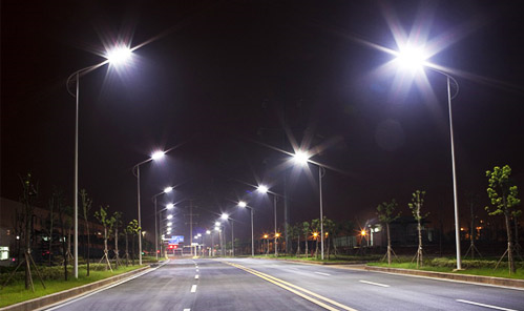
\includegraphics[scale=0.6]{image/road.png}}

\end{frame}


\part{2}
\begin{frame}[t]{Вопросы}
\vspace{0.7cm}
\center{
\includegraphics[scale=0.3]{image/questions.jpg}} \\
\end{frame}

\end{document}